\documentclass{standalone}

\usepackage{tikz}
\usetikzlibrary{positioning, calc, backgrounds, fit, shapes}

% mcs --- memory consistency system. #1: name (an id number) for the node (also used in node text); #2: position
\newcommand{\mcs}[2]{\node (#1) [rectangle split,  rectangle split parts = 3, 
  rectangle split part fill = {lightgray, white, white}, draw, text width = 2.5cm, align = center] at (#2) 
  {Replica $r_{#1}$: \nodepart{two} local registers \nodepart{three} algorithm};}

\begin{document}

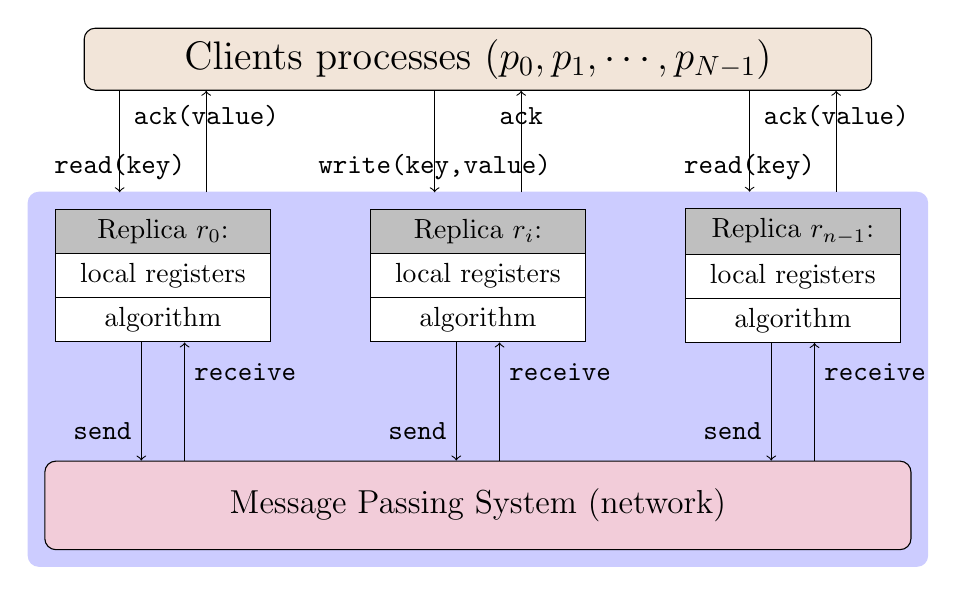
\begin{tikzpicture}
  \mcs{0}{0,0}
   \mcs{i}{4,0}
  \mcs{n-1}{8,0}
  
  % mps --- message-passing system
  \node (mps) [draw, below = 1.5cm of i, font = \large, inner sep = 10pt, minimum width = 11cm, rounded corners, fill = purple!20] {Message Passing System (network)};
  
  % mcs to mps
  \foreach \x in {0, i, n-1}
  {
  \coordinate (left) at ($ (\x.south west) ! 0.8 ! (\x.south) $);
  \coordinate (right) at ($ (\x.south east) ! 0.8 ! (\x.south) $);
  \draw[->] (left) to node[left, near end] {\texttt{send}} (left |- mps.north);
  \draw[<-] (right) to node[right, near start] {\texttt{receive}} (right |- mps.north);
  }
  
  % users 
   \node (user) [rectangle, rounded corners, fill = brown!20, draw, above = 1.5cm of i, font = 
   \Large, inner sep = 4pt, minimum width = 10cm] {Clients processes ($p_0, p_1, \cdots, 
     p_{N-1}$)};

  % background for dsm
  \begin{pgfonlayer}{background}
    \node (dsm) [fill = blue!20, fit = (0) (n-1) (mps), inner sep = 6pt, rounded corners] {};
  \end{pgfonlayer}
  
  % users to mcs (or dsm) (6pt is the inner sep for dsm)

  % client 0 and client n-1 read 
  \foreach \x in {0,  n-1}
  {
  \coordinate (left) at ($ (\x.north west) ! 0.6 ! (\x.north) + (0, 6pt) $);
  \coordinate (right) at ($ (\x.north east) ! 0.6 ! (\x.north) + (0, 6pt) $);
  \draw[<-] (left) to node[near start] {\texttt{read(key)}} (left |- user.south);
  \draw[->] (right) to node[near end] {\texttt{ack(value)}} (right |- user.south);
  }   

  % client i writes
  \foreach \x in {i}
  {
  \coordinate (left) at ($ (\x.north west) ! 0.6 ! (\x.north) + (0, 6pt) $);
  \coordinate (right) at ($ (\x.north east) ! 0.6 ! (\x.north) + (0, 6pt) $);
  \draw[<-] (left) to node[near start] {\texttt{write(key,value)}} (left |- user.south);
  \draw[->] (right) to node[near end] {\texttt{ack}} (right |- user.south);
  }
\end{tikzpicture}

\end{document}
